
\section{Architecture Integration}

\subsection{Model Support}

\begin{table}[H]
\centering
\small
\begin{tabular}{llllllll}
\toprule
\textbf{Model} & \textbf{Layers} & \textbf{$d$} & \textbf{$H$} & \textbf{$H_{kv}$} & \textbf{Attention} & \textbf{Nested?} & \textbf{Conv1D?} \\
\midrule
DistilBERT-base & 6 & 768 & 12 & 12 & Flat & No & No \\
RoBERTa-base & 12 & 768 & 12 & 12 & Nested & Yes & No \\
GPT-2 & 12 & 768 & 12 & 12 & Causal & No & Yes \\
Qwen3.5-0.8B & 24 & 1024 & 8 & 2 & GQA+RoPE & No & No \\
\bottomrule
\end{tabular}
\end{table}

\subsection{DistilBERT (Flat)}

\begin{lstlisting}
distilbert.transformer.layer.0.attention
+-- q\_lin  (Linear 768 $\to$ 768)
+-- k\_lin  (Linear 768 $\to$ 768)
+-- v\_lin  (Linear 768 $\to$ 768)
+-- out\_lin (Linear 768 $\to$ 768)
\end{lstlisting}

All four are \texttt{nn.Linear}. \textbf{Direct factorization}, no special handling.

\texttt{is\_nested\_encoder = False} because \texttt{out\_lin} is inside the attention 
module and must be applied by MinimalNOVA.

\subsection{RoBERTa (Nested)}

\begin{lstlisting}
roberta.encoder.layer.0.attention
+-- self
|   +-- query  (Linear 768 $\to$ 768)
|   +-- key    (Linear 768 $\to$ 768)
|   +-- value  (Linear 768 $\to$ 768)
+-- output
    +-- dense  (Linear 768 $\to$ 768)   # $\leftarrow$ output projection OUTSIDE
\end{lstlisting}

\textbf{Critical:} \texttt{output.dense} sits \textbf{outside} \texttt{self}. When MinimalNOVA 
replaces \texttt{self}, the outer \texttt{output.dense} must still apply.

\texttt{is\_nested\_encoder = True} because:
\begin{itemize}
\item MinimalNOVA returns the attention \textbf{context} (before output projection).
\item The outer \texttt{output.dense} applies the projection.

\end{itemize}
If we incorrectly set \texttt{is\_nested\_encoder = False}, \texttt{output.dense} is applied 
\textbf{twice}, causing scale collapse.

\subsection{GPT-2 (Causal Conv1D)}

\begin{lstlisting}
transformer.h.0.attn
+-- c\_attn  (Conv1D 768 $\to$ 2304)   # $\leftarrow$ FUSED Q, K, V
+-- c\_proj  (Conv1D 768 $\to$ 768)    # $\leftarrow$ output projection
\end{lstlisting}

\textbf{Two challenges:}

\begin{enumerate}
\item \textbf{Fused c\_attn.} Q, K, V are stored in one matrix. We split it:
\end{enumerate}
\begin{lstlisting}
   w = src.c\_attn.weight.data.clone()
   if "Conv1D" in type(src.c\_attn).\_\_name\_\_:
       w = w.t()   # (in, out) $\to$ (out, in)
   q\_w, k\_w, v\_w = w.chunk(3, dim=0)
\end{lstlisting}

\begin{enumerate}
\item \textbf{Conv1D orientation.} HuggingFace's \texttt{Conv1D} stores weights as
  \texttt{(in, out)}, opposite to \texttt{nn.Linear}. We detect this via:
\end{enumerate}
\begin{lstlisting}
   is\_conv1d = hasattr(module, "nf") or "Conv1D" in type(module).\_\_name\_\_
   if is\_conv1d:
       w = w.t()
\end{lstlisting}

\texttt{is\_nested\_encoder = False} because \texttt{c\_proj} is applied by our module.

\subsection{Qwen3.5 (GQA + RoPE)}

\begin{lstlisting}
model.layers.0.self\_attn
+-- q\_proj  (Linear 1024 $\to$ 2048)   # H * d\_h = 8 * 256
+-- k\_proj  (Linear 1024 $\to$ 512)    # H\_kv * d\_h = 2 * 256
+-- v\_proj  (Linear 1024 $\to$ 512)
+-- o\_proj  (Linear 2048 $\to$ 1024)
\end{lstlisting}

\textbf{GQA handling:} $H_{kv} = 2 < H = 8$. K and V projections are narrower. 
MinimalNOVA factorizes each at its natural dimension. During forward:

\begin{lstlisting}
if self.num\_kv\_heads \textless{} self.num\_heads:
    K = repeat\_kv(K, self.kv\_repeat)   # (B, 2, N, 256) $\to$ (B, 8, N, 256)
    V = repeat\_kv(V, self.kv\_repeat)
\end{lstlisting}

\textbf{RoPE handling:} Qwen applies RoPE after projection. MinimalNOVA preserves 
this via \texttt{position\_embeddings} argument:

\begin{lstlisting}
if position\_embeddings is not None:
    cos, sin = position\_embeddings
    Q, K = apply\_rotary\_pos\_emb(Q, K, cos, sin)
\end{lstlisting}

\texttt{is\_nested\_encoder = False} because \texttt{o\_proj} is inside the attention.

\subsection{The Nested Encoder Bypass}

When \texttt{is\_nested\_encoder = True}:

\begin{lstlisting}
def forward(self, ...):
    ...
    context = torch.matmul(attn\_weights, V)
    context = context.transpose(1, 2).contiguous().view(B, N, self.all\_head\_size)
    
    if self.is\_nested\_encoder:
        return context, attn\_weights   # $\leftarrow$ Raw context, no out\_proj
    else:
        output = self.out\_proj(context)
        return output, attn\_weights
\end{lstlisting}

The outer \texttt{BertSelfOutput.dense} then applies the projection.

\subsection{Injection Algorithm}

\textbf{Algorithm 2:} Inject MinimalNOVA into a full model
\begin{lstlisting}
Input:  model M, rank\_cap r\_max, energy  
Output: M' with all attention blocks factorized

1:  layer\_list $\leftarrow$ find\_transformer\_layers(M)
2:  # Pre-test on first layer
3:  test\_src $\leftarrow$ get\_attention(layer\_list[0])
4:  test\_module $\leftarrow$ MinimalNOVA(cfg)
5:  try: test\_module.copy\_weights(test\_src)
6:  except: return None   # abort
7:
8:  # Inject each layer
9:  count $\leftarrow$ 0
10: for (idx, layer) in enumerate(layer\_list) do
11:     res $\leftarrow$ inject\_single(layer, idx, r\_max,  )
12:     if res is not None:
13:         count += 1
14: end for
15:
16: return M' if count \textgreater{} 0 else None
\end{lstlisting}

\subsection{Failure Modes and Fallbacks}

\begin{table}[H]
\centering
\small
\begin{tabular}{lll}
\toprule
\textbf{Failure} & \textbf{Detection} & \textbf{Response} \\
\midrule
Missing Q/K/V weights & \texttt{copy\_weights} raises & Abort \\
Near-zero Frobenius & Norm check \textless{} 1e-4 & Raise \\
Shape mismatch & \texttt{\_orient} handles & Warn and pad \\
Double injection & Class name check & Skip \\
Cross-attention & Not supported & Raise \\
\bottomrule
\end{tabular}
\end{table}

\subsection{Registry}

\begin{lstlisting}
@ATTENTION\_REGISTRY.register("minimal\_nova")
class MinimalNOVAAttention(BaseAttention):
    ...

@ATTENTION\_REGISTRY.register("minimal\_nova\_inject")
@ATTENTION\_REGISTRY.register("inject\_minimal\_nova")
def inject\_minimal\_nova(...):
    ...
\end{lstlisting}

\subsection{Compatibility with LoRA Recovery Pipeline}

MinimalNOVA integrates cleanly with the framework's LoRA recovery:

\begin{enumerate}
\item \textbf{Inject} MinimalNOVA $\to$ factorized attention with frozen base.
\item \textbf{LoRA adapters} are inside each \texttt{FactorisedLinear} (trainable).
\item \textbf{Recovery fine-tuning} trains only LoRA parameters.
\item \textbf{Evaluation} uses the fine-tuned model.

\end{enumerate}
The framework's \texttt{get\_recovery\_params} finds \texttt{lora\_A}, \texttt{lora\_B} parameters 
automatically via the naming convention.
\begin{lstlisting}

---
\end{lstlisting}

\begin{figure}[H]
\centering
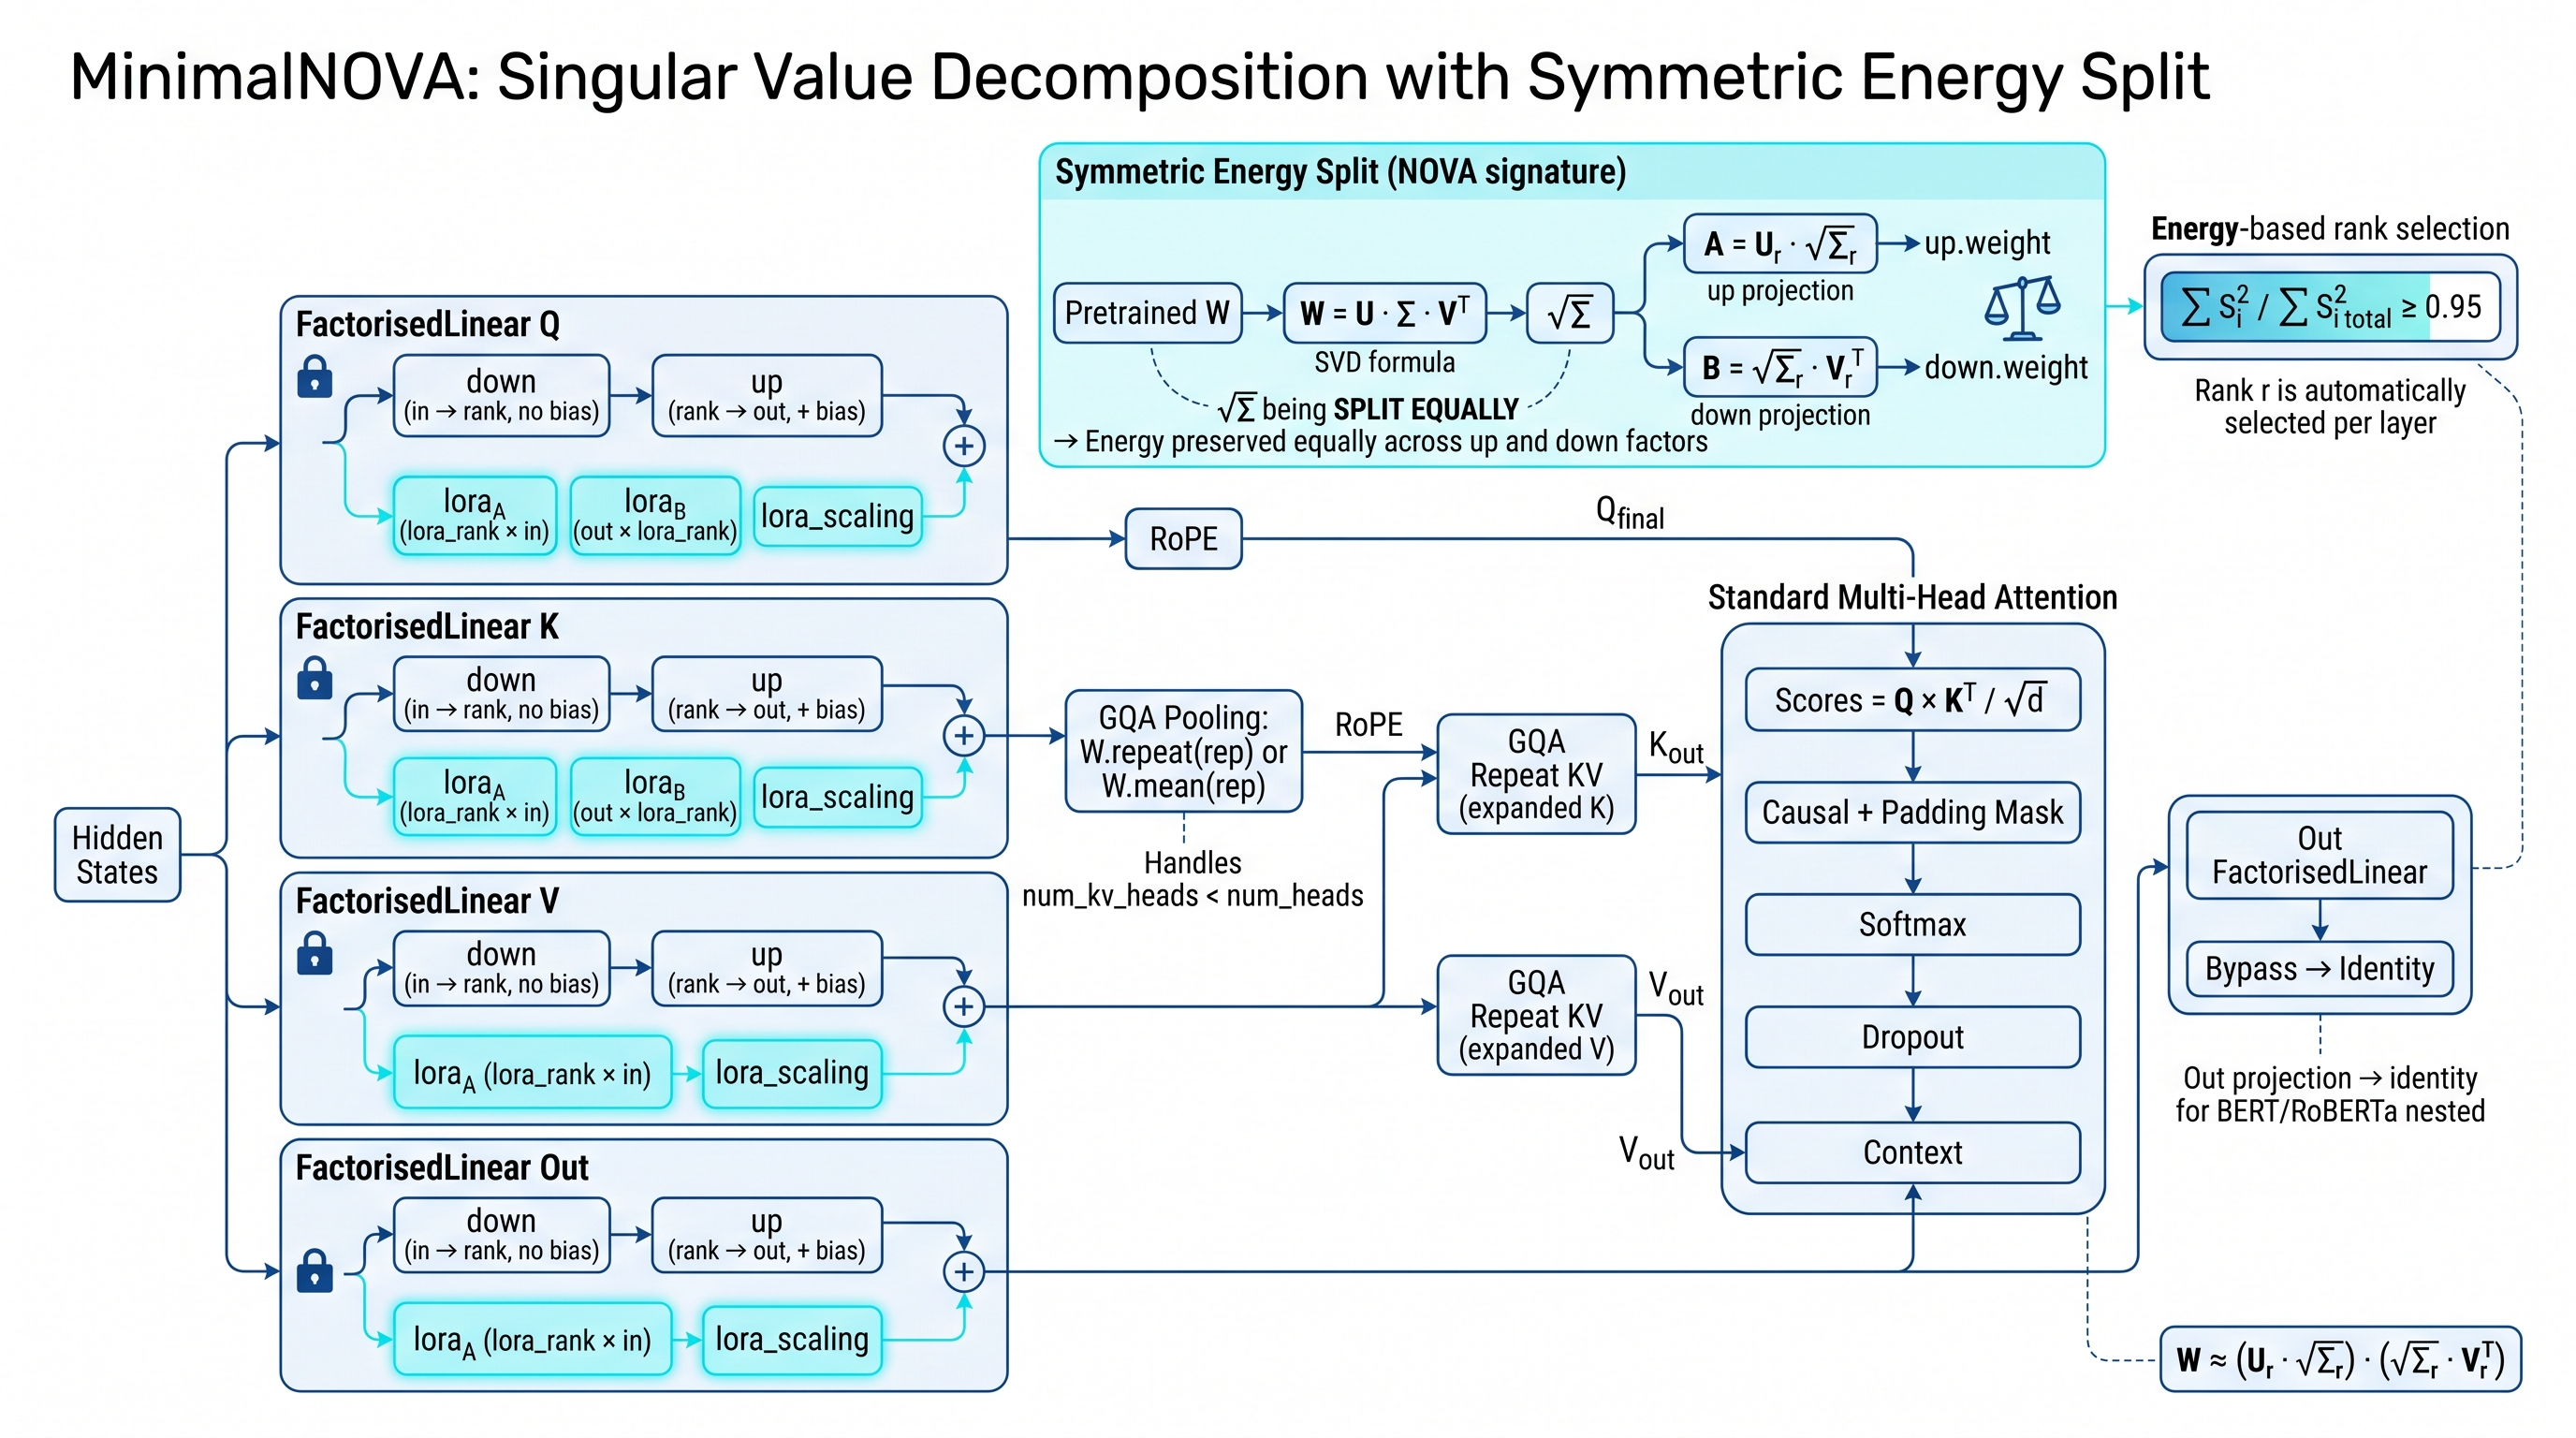
\includegraphics[width=\linewidth]{figures/architecture.jpeg}
\caption{High-level architectural diagram of minimal\_nova.}
\label{fig:arch_minimal-nova}
\end{figure}

